%%%%%%%% ICML 2020 EXAMPLE LATEX SUBMISSION FILE %%%%%%%%%%%%%%%%%

\documentclass{article}

% Recommended, but optional, packages for figures and better typesetting:
\usepackage{microtype}
\usepackage{graphicx}
\usepackage{subfigure}
\usepackage{booktabs} % for professional tables

% hyperref makes hyperlinks in the resulting PDF.
% If your build breaks (sometimes temporarily if a hyperlink spans a page)
% please comment out the following usepackage line and replace
% \usepackage{icml2020} with \usepackage[nohyperref]{icml2020} above.
\usepackage{hyperref}

% Attempt to make hyperref and algorithmic work together better:
\newcommand{\theHalgorithm}{\arabic{algorithm}}

% Use the following line for the initial blind version submitted for review:
\usepackage{icml2020}

% If accepted, instead use the following line for the camera-ready submission:
%\usepackage[accepted]{icml2020}

% The \icmltitle you define below is probably too long as a header.
% Therefore, a short form for the running title is supplied here:
\icmltitlerunning{Missing the Point}

\begin{document}

\twocolumn[
\icmltitle{Missing the Point: Non-Convergence in Iterative Imputation Algorithms}

% It is OKAY to include author information, even for blind
% submissions: the style file will automatically remove it for you
% unless you've provided the [accepted] option to the icml2020
% package.

% List of affiliations: The first argument should be a (short)
% identifier you will use later to specify author affiliations
% Academic affiliations should list Department, University, City, Region, Country
% Industry affiliations should list Company, City, Region, Country

% You can specify symbols, otherwise they are numbered in order.
% Ideally, you should not use this facility. Affiliations will be numbered
% in order of appearance and this is the preferred way.
\icmlsetsymbol{equal}{*}

\begin{icmlauthorlist}
\icmlauthor{Hanne I.~Oberman}{UU}
\icmlauthor{Stef van~Buuren}{UU}
\icmlauthor{Gerko Vink}{UU}
\end{icmlauthorlist}

\icmlaffiliation{UU}{Department of Methodology and Statistics, Utrecht University, Utrecht, The Netherlands}

\icmlcorrespondingauthor{Hanne Oberman}{h.i.oberman@uu.nl}

% You may provide any keywords that you
% find helpful for describing your paper; these are used to populate
% the "keywords" metadata in the PDF but will not be shown in the document
\icmlkeywords{Iterative imputation, MICE, non-convergence}

\vskip 0.3in
]

% this must go after the closing bracket ] following \twocolumn[ ...

% This command actually creates the footnote in the first column
% listing the affiliations and the copyright notice.
% The command takes one argument, which is text to display at the start of the footnote.
% The \icmlEqualContribution command is standard text for equal contribution.
% Remove it (just {}) if you do not need this facility.

%\printAffiliationsAndNotice{}  % leave blank if no need to mention equal contribution
\printAffiliationsAndNotice{\icmlEqualContribution} % otherwise use the standard text.

\begin{abstract}
Iterative imputation is a popular tool to accommodate missing data. While it is widely accepted that valid inferences can be obtained with this technique, these inferences all rely on algorithmic convergence. There is no consensus on how to evaluate the convergence properties of the method. This paper provides insight into identifying non-convergence in iterative imputation algorithms. Our study found that---in the cases considered---inferential validity was achieved after five to ten iterations, much earlier than indicated by diagnostic methods. We conclude that it never hurts to iterate longer, but such calculations hardly bring added value.
\end{abstract}

\section{Introduction}
\label{intro}

A popular method to accommodate missing data is to \textit{impute} (i.e., `fill in') the missing values in an incomplete dataset. It is widely accepted that imputation techniques such as multiple imputation \citep[MI;][]{rubin76} can yield statistically valid inferences. The validity of these inferences relies on the method through which imputations are obtained---often iterative algorithms. Iterative imputation algorithms are employed in e.g., $\mathtt{SPSS}$, $\mathtt{Stata}$, and the $\mathtt{R}$ packages $\mathtt{MI}$, and $\mathtt{mice}$. \textit{[Or use:} Convergence of the algorithm used to solve the missing data problem is a topic that has not received much attention but is ever so important, as most imputation software packages draw inference from iterative imputation procedures.]

With iterative imputation, the validity of the inference depends on the state-space of the algorithm at the final iteration. This introduces a potential threat to the validity of the imputations: What if the algorithm has not converged? Are the imputations then to be trusted? And can we rely on the inference obtained on the completed data?

These remain open questions since the convergence properties of iterative imputation algorithms have not been systematically studied \citep{buur18}.\footnote{If the algorithm does not reach convergence, ``the imputed datasets will not be truly independent and the variability among them may understate the true levels of missing-data uncertainty'' (Schafer and Olsen, p. 556).} There is no scientific consensus on how to evaluate the convergence of imputation algorithms \citep{zhu15, taka17}. Moreover, the behavior of such algorithms under certain default imputation models (e.g., `predictive mean matching') is an entirely open question \citep{murr18}. Therefore, algorithmic convergence should be monitored carefully.

The current practice of visually inspecting imputations may be undesirable for several reasons: 1) it may be challenging to the untrained eye, 2) only severely pathological cases of non-convergence may be diagnosed, and 3) there is not an objective measure that quantifies convergence \citep[\(\S\) 6.5.2]{buur18}. On top of that, the recommended parameters to inspect may be insufficient. The parameters are scalar summaries of the state-space of the algorithm. They are either univariate, or depend on the substantive model of interest. Apparent convergence of a univariate parameter does not guarantee convergence of the multivariate state-space of the algorithm. And with a model-dependent statistic there is no guarantee that the algorithm is converged \textit{enough} for other models of scientific interest. Additionally, model-dependency negates an important advantage of MI: solving the missing data problem separately from the scientific problem.

Therefore, we propose a novel parameter to inspect. We use this parameter to identify non-convergence with two quantitative diagnostic methods. We use model-based simulation to investigate the plausibility of identifiers for non-convergence for iterative imputation algorithms and provide guidelines for empirical research. For reasons of brevity, we only focus on the iterative imputation algorithm implemented in the popular \texttt{mice} package in \texttt{R} \citep{mice, R}. \textit{[Provide notation here? E.g., the number of imputations, iterations, etc.]}


\section{Methods}
\label{methods}

\subsection{Diagnostic Methods}
We consider several sets of diagnostic methods to identify non-convergence in the iterative imputation algorithm. Each method is a combination of a parameter that summarizes the state-space of the algorithm, $\theta$, and an identifier. As $\theta$s we use the default parameters of the \texttt{MICE} algorithm (i.e., the univariate $\theta$s chain means and chain variances), a model-dependent user-specified multivariate parameter $Q$, and a novel parameter: $\lambda_1$. $\lambda_{1}$ has the appealing property that it is not dependent on the model of scientific interest, yet still summarizes the multivariate state-space of the algorithm.

We define $\lambda_{1}$ as the first eigenvalue of the variance-covariance matrix of the completed data.\footnote{By definition, this is equal to the variance of the first component of the principal component analylis (PCA) solution on the same data.} For each imputation $\ell$, let $\lambda_{1, \ell} \geq \lambda_{2, \ell} \geq ... \geq \lambda_{j, \ell}$ be the eigenvalues of the variance-covariance matrix $S_{\ell}$, where $\ell = 1, ..., m$. Since the eigenvalues of a variance-covariance matrix summarize the total set of covariances in the data, $\lambda_1$ captures the multivariate nature of the completed data without imposing a substantive model of interest. 

The identifiers are as recommended by e.g. \cite{cowl96}, namely the potential scale reduction factor $\widehat{R}$ and autocorrelation. $\widehat{R}$ is also known as the `Gelman-Rubin statistic' after the original paper \cite{gelm92}. We use a recently proposed adapted version of $\widehat{R}$ \citep{veht19}. We diagnose non-convergence if $\widehat{R}$-values exceed a certain diagnostic threshold. The thresholds under consideration are the traditional threshold $\widehat{R}=1.2$ \citep{gelm92}, the common $\widehat{R}=1.1$ \citep{gelm13}, and the recent $\widehat{R}=1.01$ \citep{veht19}. 

We diagnose non-convergence with autocorrelation when the correlation between two subsequent $\theta$-values within the same chain is significantly different from zero \citep[p.~147, p.~42]{lync07, hynd18}.

\subsection{Simulation Study}
We investigate non-convergence of the iterative imputation algorithm implemented in the $\mathtt{R}$ package $\mathtt{mice}$ through model-based simulation. The simulation set-up is summarized in pseudo-code (see Algorithm \ref{alg:setup}). The complete script and technical details are available from \href{https://github.com/hanneoberman/MissingThePoint}{github.com/hanneoberman/MissingThePoint}. \textit{[Define conditions here somewhere, and $p_{\rm inc}$and $T$.]}

\begin{algorithm}
   \caption{Simulation set-up}
   \label{alg:setup}
\begin{algorithmic}
\STATE Simulate data 
\REPEAT 
\FOR {$p_{\rm inc} = .05, .25, .50, .75, .95$ (missingness conditions)}
  \STATE Create missingness
  \FOR {$T = 1, 2, ..., 100$ (early stopping conditions)}
   \STATE Impute missingness
   \STATE Perform analysis of scientific interest
   \STATE Compute non-convergence diagnostics 
   \STATE Pool results across imputations
   \STATE Compute performance measures
   \ENDFOR
 \ENDFOR 
 \STATE Combine outcomes of all conditions
\UNTIL{$n_{\rm sim} = 1000$ (simulation repetitions)}
\STATE Aggregate outcomes across simulation runs
\end{algorithmic}
\end{algorithm}

The aim of the simulation study is twofold: 1) to determine the effect of early stopping and missingness conditions on the validity of statistical inferences, 2) to investigate the plausibility of identifiers for non-convergence. 

We assess the validity of statistical inferences with bias, coverage rate and confidence interval width as performance measures (see @buur18 for definitions). And we evaluate the plausibility of the identifiers using the diagnostic thresholds for $\widehat{R}$ and autocorrelation (i.e., $\widehat{R}=1.2,1.1,1.01$ and the critical value for AC = 0).

\textit{[Very incomplete from here!]} We consider several quantities of scientific interest.

The statistical inference of interest is multivariate linear regression.

The data generating mechanism of the predictor space is a multivariate normal distribution



\section{Results}
\label{results}

\begin{figure*}
{\centering 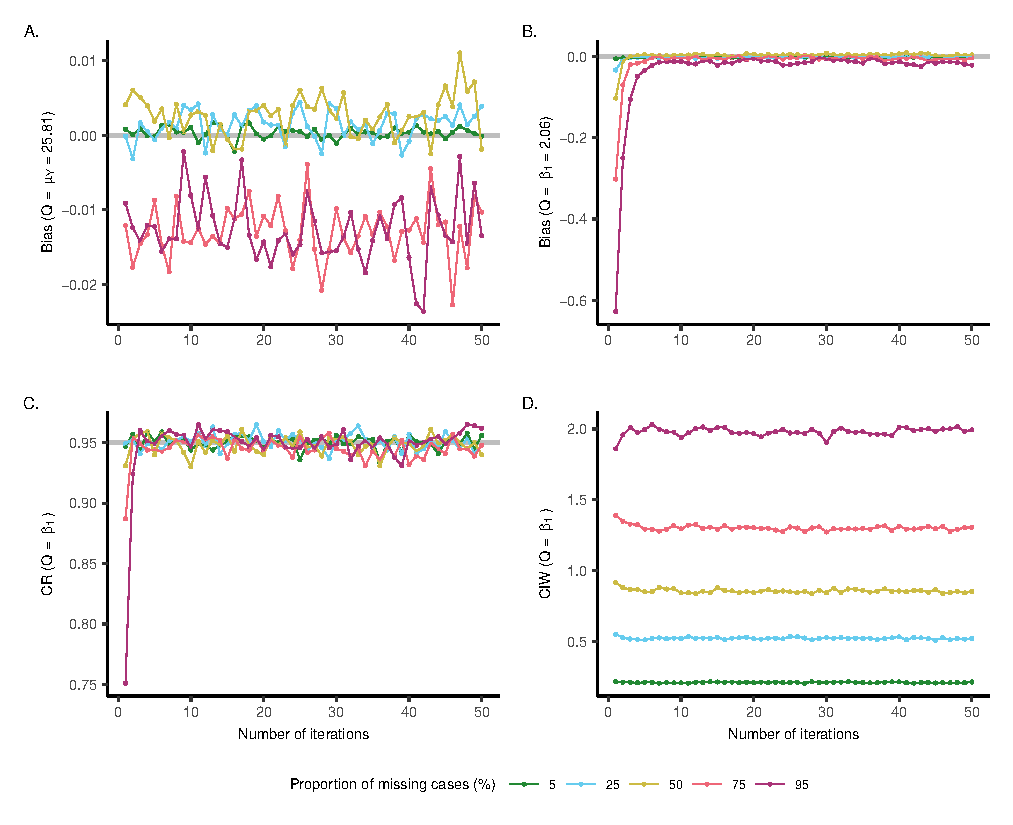
\includegraphics{Figures/estimates} 
}
\caption{Impact of non-convergence on statistical inferences. Depicted are the bias, coverage rate (CR) and confidence interval width (CIW) of the worst-performing quantities of scientific interest $Q$ in terms of bias. The gray lines represent the objectives: unbiased estimates with nominal coverage.}\label{fig:est}
\end{figure*}

Results are displayed in Figure \ref{fig:est} and \ref{fig:diag}. Simulation conditions with a high proportion of missing cases and a low number of iterations most often result in biased estimates and non-nominal coverages. 

\textit{[Copy-paste from here!]} These results demonstrate that the estimates of univariate scientific estimands \(Q\) are not impacted by early stopping of the MICE algorithm or the proportion of incomplete cases in \(y\). Unbiased estimates may be obtained after just one iteration. Multivariate estimates, by contrast, are affected by both the number of iterations and the proportion of missing cases. Completely unbiased estimates are only obtained under low to moderate missingness (\(p_{\rm inc}\leq.50\)), after at most three iterations. We observe approximately unbiased estimates after at most seven iterations (for any \(p_{\rm inc}\) considered). This implies that the algorithm produces stable, non-improving estimates when \(T\geq7\).

\begin{figure*}
{\centering 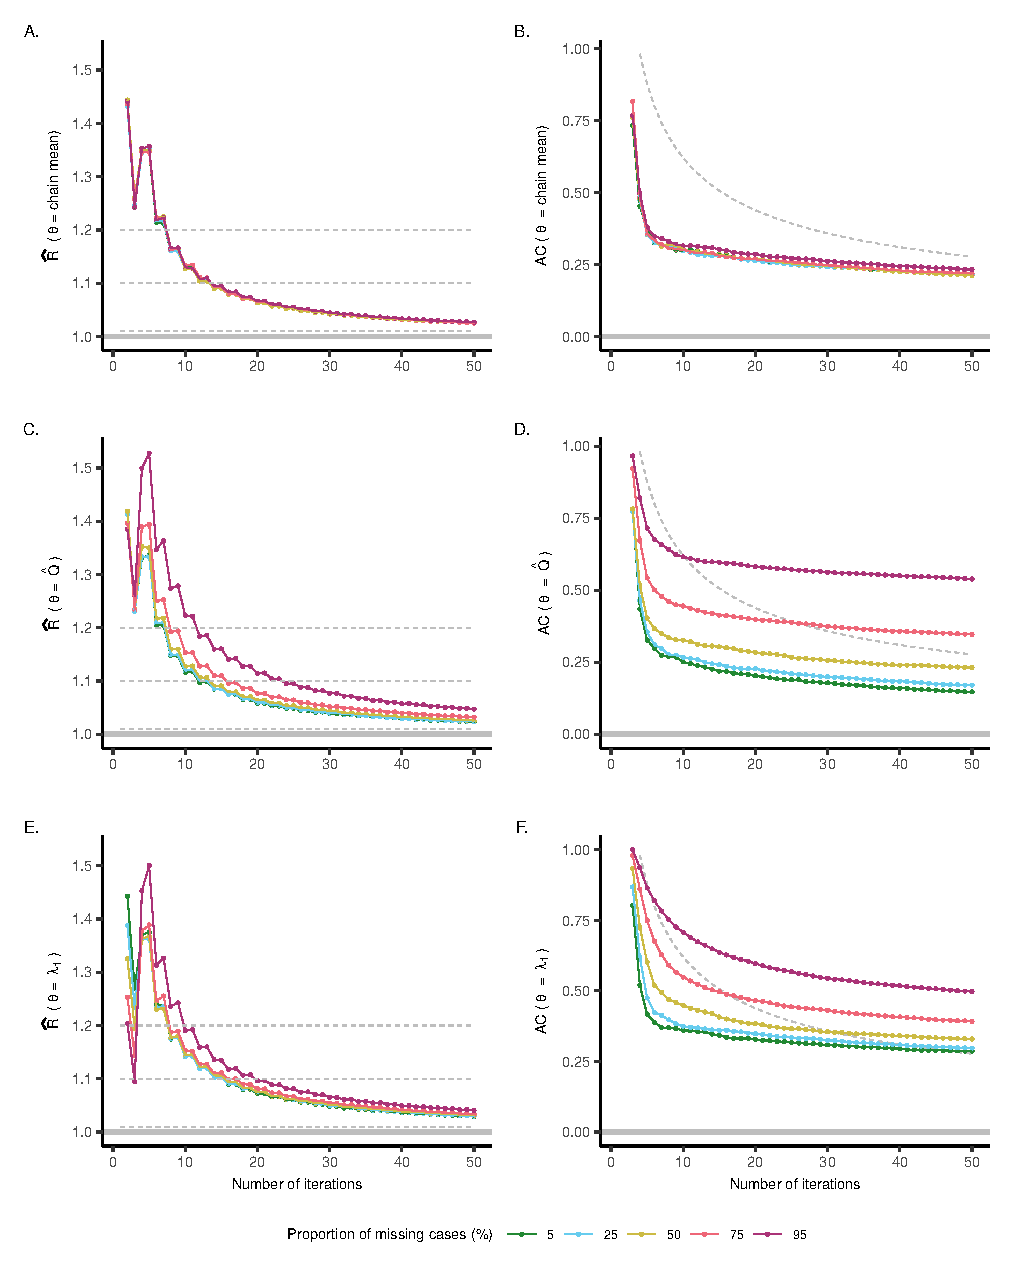
\includegraphics{Figures/diagnostics} 
}
\caption{Non-convergence identified by diagnostic methods: $\widehat{R}$ and $AC$ applied on several $\theta$s. The left-hand side of the figure contains $\widehat{R}$-values, and the right-hand side contains $AC$-values. Depicted in the rows are the scalar summaries $\theta$: chain mean, chain variance, the quantity of scientific interest $\hat{Q}$, and the first eigenvalue of the variance-covariance matrix $\lambda_1$.}\label{fig:diag}
\end{figure*}


Overall, the methods to diagnose non-convergence perform as expected: they indicate more signs of non-convergence in conditions with worse performance in terms of bias and confidence-validity. Under low to moderate missingness, it does not seem to matter on which \(\theta\) the non-convergence diagnostics are applied. If we look at complete unbiasedness, however, we notice that univariate \(\theta\)s fail to diagnose the persistent bias in conditions where \(p_{\rm inc}\geq.75\).

The number of iterations necessary to obtain approximately unbiased, confidence-valid estimates corresponds to the \(\widehat{R}\) threshold 1.2. The thresholds 1.1 and 1.01 seem too strict compared to the validity of the inferences. The threshold to diagnose significant \(AC\)-values does not appear to be appropriate in at least the current set-up, and perhaps in iterative imputation in general. A better heuristic to diagnose non-stationarity with \(AC\) may be through evaluation of the \(AC\)-values across iterations: If the values do not substantially decrease with \(T\), approximate stationarity may be concluded.





\section{Discussion}
\label{discussion}

We have shown that iterative imputation algorithms can yield correct outcomes, even when a converged state has not yet formally been reached. Any further iterations would then burn computational resources without improving the statistical inferences. Our study found that---in the cases considered---inferential validity was achieved after five to ten iterations, much earlier than indicated by the \(\widehat{R}\) and AC diagnostics. Of course, it never hurts to iterate longer, but such calculations hardly bring added value.


% In the unusual situation where you want a paper to appear in the
% references without citing it in the main text, use \nocite

\bibliography{missing_the_point}
\bibliographystyle{icml2020}




\end{document}


% This document was modified from the file originally made available by
% Pat Langley and Andrea Danyluk for ICML-2K. This version was created
% by Iain Murray in 2018, and modified by Alexandre Bouchard in
% 2019 and 2020. Previous contributors include Dan Roy, Lise Getoor and Tobias
% Scheffer, which was slightly modified from the 2010 version by
% Thorsten Joachims & Johannes Fuernkranz, slightly modified from the
% 2009 version by Kiri Wagstaff and Sam Roweis's 2008 version, which is
% slightly modified from Prasad Tadepalli's 2007 version which is a
% lightly changed version of the previous year's version by Andrew
% Moore, which was in turn edited from those of Kristian Kersting and
% Codrina Lauth. Alex Smola contributed to the algorithmic style files.
